% Diagrama de Componentes UML — SmartSupply (estado 2026-09)
\documentclass[tikz, border=14pt]{standalone}
\usepackage[utf8]{inputenc}
\usepackage[T1]{fontenc}
\usepackage{helvet}
\renewcommand{\familydefault}{\sfdefault}
\usetikzlibrary{positioning, arrows.meta, fit, backgrounds}

% Icono UML de componente en la esquina superior derecha del nodo
\tikzset{
  compicon/.style={path picture={
    \draw[line width=0.6pt, fill=white]
      ([xshift=-0.46cm, yshift=-0.10cm]path picture bounding box.north east) rectangle ++(0.36,-0.28);
    \draw[line width=0.5pt, fill=white]
      ([xshift=-0.54cm, yshift=-0.13cm]path picture bounding box.north east) rectangle ++(0.16,-0.08);
    \draw[line width=0.5pt, fill=white]
      ([xshift=-0.54cm, yshift=-0.26cm]path picture bounding box.north east) rectangle ++(0.16,-0.08);
  }},
  comp/.style={draw, line width=0.8pt, fill=white, align=left, anchor=north,
    text width=#1, inner sep=6pt, compicon},
  comp/.default=4.9cm,
  sub/.style={draw, line width=0.9pt, dashed, rounded corners=4pt, inner sep=10pt},
  dep/.style={line width=0.8pt, dashed, -{Latex[length=2.3mm]}},
  arr/.style={line width=0.8pt, -{Latex[length=2.3mm]}},
  lbl/.style={font=\scriptsize\sffamily, fill=white, inner sep=1.2pt, align=center},
}
\newcommand{\st}{{\footnotesize\itshape\textless\textless component\textgreater\textgreater}\\}
\newcommand{\sm}[1]{{\footnotesize\color{black!70}#1}}

\begin{document}
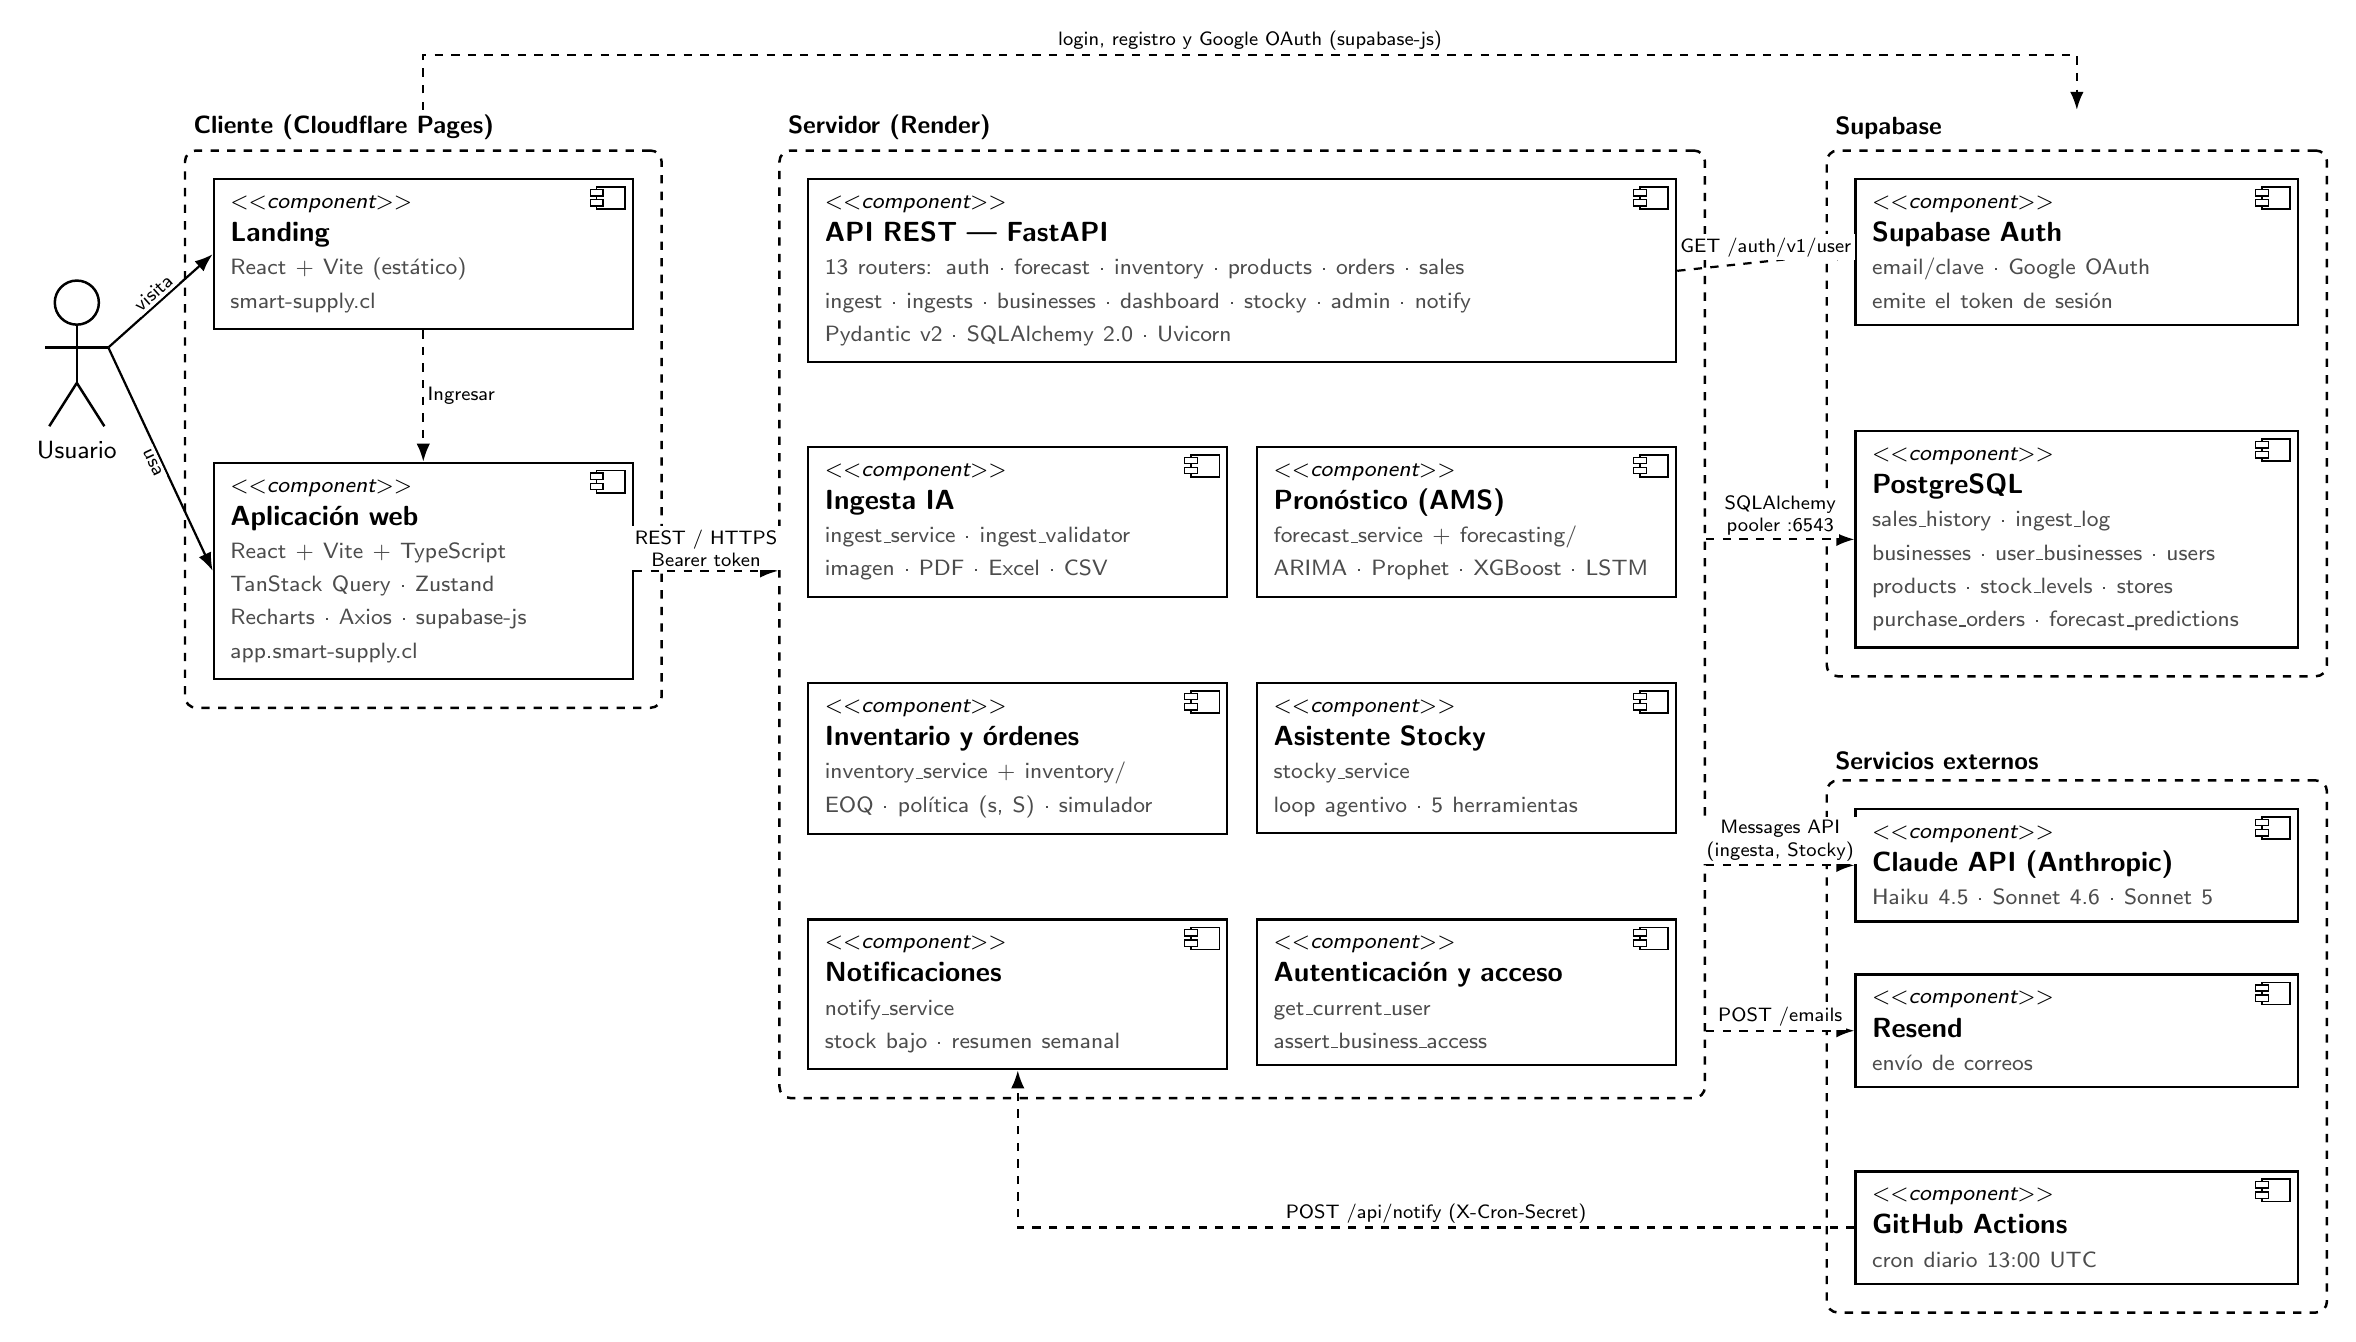
\begin{tikzpicture}[font=\sffamily]

% ── Cliente ─────────────────────────────────────────────────
\node[comp] (landing) at (2.6, 0) {\st\textbf{Landing}\\
  \sm{React + Vite (estático)}\\ \sm{smart-supply.cl}};
\node[comp] (app) at (2.6, -3.6) {\st\textbf{Aplicación web}\\
  \sm{React + Vite + TypeScript}\\ \sm{TanStack Query · Zustand}\\
  \sm{Recharts · Axios · supabase-js}\\ \sm{app.smart-supply.cl}};

% ── Servidor (Render) ───────────────────────────────────────
\node[comp=10.6cm] (api) at (13.0, 0) {\st\textbf{API REST --- FastAPI}\\
  \sm{13 routers: auth · forecast · inventory · products · orders · sales}\\
  \sm{ingest · ingests · businesses · dashboard · stocky · admin · notify}\\
  \sm{Pydantic v2 · SQLAlchemy 2.0 · Uvicorn}};

\node[comp] (ing) at (10.15, -3.4) {\st\textbf{Ingesta IA}\\
  \sm{ingest\_service · ingest\_validator}\\ \sm{imagen · PDF · Excel · CSV}};
\node[comp] (fc) at (15.85, -3.4) {\st\textbf{Pronóstico (AMS)}\\
  \sm{forecast\_service + forecasting/}\\ \sm{ARIMA · Prophet · XGBoost · LSTM}};
\node[comp] (inv) at (10.15, -6.4) {\st\textbf{Inventario y órdenes}\\
  \sm{inventory\_service + inventory/}\\ \sm{EOQ · política (s, S) · simulador}};
\node[comp] (sto) at (15.85, -6.4) {\st\textbf{Asistente Stocky}\\
  \sm{stocky\_service}\\ \sm{loop agentivo · 5 herramientas}};
\node[comp] (not) at (10.15, -9.4) {\st\textbf{Notificaciones}\\
  \sm{notify\_service}\\ \sm{stock bajo · resumen semanal}};
\node[comp] (aut) at (15.85, -9.4) {\st\textbf{Autenticación y acceso}\\
  \sm{get\_current\_user}\\ \sm{assert\_business\_access}};

% ── Supabase ────────────────────────────────────────────────
\node[comp=5.2cm] (sauth) at (23.6, 0) {\st\textbf{Supabase Auth}\\
  \sm{email/clave · Google OAuth}\\ \sm{emite el token de sesión}};
\node[comp=5.2cm] (pg) at (23.6, -3.2) {\st\textbf{PostgreSQL}\\
  \sm{sales\_history · ingest\_log}\\ \sm{businesses · user\_businesses · users}\\
  \sm{products · stock\_levels · stores}\\ \sm{purchase\_orders · forecast\_predictions}};

% ── Servicios externos ──────────────────────────────────────
\node[comp=5.2cm] (claude) at (23.6, -8.0) {\st\textbf{Claude API (Anthropic)}\\
  \sm{Haiku 4.5 · Sonnet 4.6 · Sonnet 5}};
\node[comp=5.2cm] (resend) at (23.6, -10.1) {\st\textbf{Resend}\\ \sm{envío de correos}};
\node[comp=5.2cm] (gha) at (23.6, -12.6) {\st\textbf{GitHub Actions}\\ \sm{cron diario 13:00 UTC}};

% ── Subsistemas ─────────────────────────────────────────────
\begin{scope}[on background layer]
  \node[sub, fit=(landing)(app)] (sCli) {};
  \node[sub, fit=(api)(ing)(fc)(inv)(sto)(not)(aut)] (sSrv) {};
  \node[sub, fit=(sauth)(pg)] (sSup) {};
  \node[sub, fit=(claude)(resend)(gha)] (sExt) {};
\end{scope}
\foreach \n/\t in {sCli/Cliente (Cloudflare Pages), sSrv/Servidor (Render), sSup/Supabase, sExt/Servicios externos} {
  \node[font=\small\sffamily\bfseries, anchor=south west] at (\n.north west) {\t};
}

% ── Usuario ─────────────────────────────────────────────────
\begin{scope}[shift={(-1.8,-2.2)}, line width=0.9pt]
  \draw (0,0.62) circle (0.28);
  \draw (0,0.34) -- (0,-0.40);
  \draw (-0.40,0.05) -- (0.40,0.05);
  \draw (0,-0.40) -- (-0.35,-0.95);
  \draw (0,-0.40) -- (0.35,-0.95);
  \node[font=\small\sffamily] at (0,-1.25) {Usuario};
\end{scope}
\coordinate (user) at (-1.4,-2.15);

% ── Relaciones ──────────────────────────────────────────────
\draw[arr] (user) -- (landing.west) node[midway, lbl, above, sloped] {visita};
\draw[arr] (user) -- (app.west) node[midway, lbl, below, sloped] {usa};
\draw[dep] (landing) -- (app) node[midway, lbl, right] {Ingresar};

\draw[dep] (app.east) -- (sSrv.west |- app.east)
  node[midway, lbl, above] {REST / HTTPS\\Bearer token};
\draw[dep] ([yshift=5mm]sCli.north) -- ++(0,0.7) -| ([yshift=5mm]sSup.north)
  node[pos=0.25, lbl, above] {login, registro y Google OAuth (supabase-js)};

\draw[dep] (api.east) -- (sauth.west) node[midway, lbl, above] {GET /auth/v1/user};
\draw[dep] (sSrv.east |- pg.west) -- (pg.west) node[midway, lbl, above] {SQLAlchemy\\pooler :6543};
\draw[dep] (sSrv.east |- claude.west) -- (claude.west) node[midway, lbl, above] {Messages API\\(ingesta, Stocky)};
\draw[dep] (sSrv.east |- resend.west) -- (resend.west) node[midway, lbl, above] {POST /emails};
\draw[dep] (gha.west) -| (not.south) node[pos=0.25, lbl, above] {POST /api/notify (X-Cron-Secret)};

\end{tikzpicture}
\end{document}
